\documentclass[10pt,letterpaper]{article}
\usepackage[utf8]{inputenc}
\usepackage{amsmath,amssymb}
\usepackage[left=30mm,right=30mm,top=20mm,bottom=20mm,
  headheight=14pt,headsep=18pt]{geometry}
\usepackage{enumitem,fancyhdr,tikz}
\usetikzlibrary{arrows.meta}

\setlength{\parindent}{0pt}
\setlist[enumerate,1]{label=\arabic*.,leftmargin=25pt,itemsep=10pt,topsep=6pt,parsep=0pt}
\setlist[enumerate,2]{label=(\alph*),leftmargin=18pt,itemsep=4pt,topsep=4pt,parsep=0pt}
\newcommand{\R}{\mathbb{R}}
\pagestyle{fancy}
\fancyhf{}
\fancyhead[L]{\small ETS Kalkulus I 2025}
\fancyhead[R]{\small Hal. \thepage}
\renewcommand{\headrulewidth}{0.4pt}
\renewcommand{\footrulewidth}{0pt}

\begin{document}

% Kelompok 1: lima soal
\begin{enumerate}

  % Soal 1
  \item Dapatkan penyelesaian dari pertidaksamaan
        \[
          \frac{x^2-x-12}{x^2+3x-10}\ge0.
        \]

        % Soal 2
  \item \begin{enumerate}
          \item Dapatkan kemiringan garis $l$ yang melalui $(0,0)$ dan $(-2,1)$.
          \item Jika garis $l$ tegak lurus dengan garis yang menyinggung lingkaran
                yang berpusat di $(0,0)$ dan jari-jari $\sqrt5$ di titik $(-2,1)$,
                maka dapatkan persamaan garis singgung lingkaran tersebut.
        \end{enumerate}

        % Soal 3
  \item Tuliskan rumus turunan dari $f\cdot g$:
        \[
          \frac{d}{dx}\bigl(f(x)g(x)\bigr).
        \]
        Selanjutnya dapatkan turunan dari $f\cdot g$ jika diketahui
        \[
          f(x)=3x^3-7x\quad\text{dan}\quad g(x)=3-2x^3.
        \]

        % Soal 4
  \item Dapatkan
        \[
          \lim_{x\to3}\frac{\sqrt{3x+7}-4}{x-3}.
        \]

        % Soal 5
  \item Diberikan fungsi
        \[
          f(x)=\frac1{x-1}\quad\text{dan}\quad g(x)=x^2.
        \]
        \begin{enumerate}
          \item Dapatkan $(f\circ g)(x)$.
          \item Jika diketahui $(p\circ g)(x)=x^2-3$, dapatkan $p(x)$.
        \end{enumerate}

\end{enumerate}

\newpage
\begingroup
\fontsize{10.95}{13.5}\selectfont
\setlength{\parskip}{3pt}
\setlist[enumerate,1]{label=\arabic*.,leftmargin=25pt,itemsep=14pt,topsep=6pt,parsep=3pt}
\setlist[enumerate,2]{label=(\alph*),leftmargin=18pt,itemsep=8pt,topsep=5pt,parsep=3pt}
\textbf{\large Pembahasan}\par\medskip
\begin{enumerate}

  % Pembahasan soal 1
  \item Penyebut pecahan tidak boleh nol.
        Faktorkan pembilang dan penyebut:
        \[
          \frac{x^2-x-12}{x^2+3x-10}
          =\frac{(x-4)(x+3)}{(x+5)(x-2)},\qquad x\ne-5,\ 2.
        \]
        Pembilang nol pada $x=-3$ dan $x=4$.
        Keempat titik $-5,-3,2,4$ membagi garis bilangan menjadi lima selang.
        Tentukan tanda tiap faktor pada setiap selang:
        \[
          \begin{array}{c|ccccc}
            x              & (-\infty,-5) & (-5,-3) & (-3,2) & (2,4) & (4,\infty) \\ \hline
            x-4            & -            & -       & -      & -     & +          \\
            x+3            & -            & -       & +      & +     & +          \\
            x+5            & -            & +       & +      & +     & +          \\
            x-2            & -            & -       & -      & +     & +          \\ \hline
            \text{pecahan} & +            & -       & +      & -     & +
          \end{array}
        \]
        Soal meminta nilai pecahan tak negatif, sehingga pilih selang bertanda positif.
        Nilai $-3$ dan $4$ juga termasuk karena menghasilkan pecahan nol.
        Nilai $-5$ dan $2$ tetap dikeluarkan karena penyebutnya nol.
        Jadi,
        \[
          \boxed{\mathrm{HP}=(-\infty,-5)\cup[-3,2)\cup[4,\infty)}.
        \]

        % Pembahasan soal 2
  \item \begin{enumerate}
          \item Gradien adalah perbandingan perubahan koordinat $y$ dan koordinat $x$.
                Gunakan kedua titik pada garis $l$:
                \[
                  m_l=\frac{1-0}{-2-0}=\boxed{-\frac12}.
                \]

          \item Garis $l$ menghubungkan pusat lingkaran dengan titik singgung $(-2,1)$.
                Jadi, garis ini merupakan garis yang memuat jari-jari lingkaran.
                Garis singgung tegak lurus terhadap jari-jari di titik singgung.

                Jika gradien garis singgung adalah $m_t$, maka
                \[
                  m_lm_t=-1\quad\Longrightarrow\quad
                  -\frac12m_t=-1\quad\Longrightarrow\quad m_t=2.
                \]
                Garis singgung melalui $(-2,1)$.
                Masukkan titik dan gradiennya ke bentuk $y-y_0=m(x-x_0)$:
                \begin{align*}
                  y-1 & =2\bigl(x-(-2)\bigr), \\
                  y-1 & =2x+4,                \\
                  y   & =2x+5.
                \end{align*}
                Jadi, persamaan garis singgungnya $\boxed{y=2x+5}$.
                Titik singgungnya memang berada pada lingkaran karena $(-2)^2+1^2=5$.
        \end{enumerate}

        \newpage

        % Pembahasan soal 3
  \item Gunakan aturan turunan hasil kali:
        \[
          \boxed{\frac{d}{dx}\bigl(f(x)g(x)\bigr)=f'(x)g(x)+f(x)g'(x)}.
        \]
        Artinya, turunkan faktor pertama dan biarkan faktor kedua tetap.
        Lalu tambahkan hasil kali faktor pertama dengan turunan faktor kedua.
        Turunan masing-masing fungsi adalah
        \[
          f'(x)=9x^2-7,\qquad g'(x)=-6x^2.
        \]
        Substitusikan ke aturan hasil kali:
        \begin{align*}
          (f\cdot g)'(x)
           & =(9x^2-7)(3-2x^3)+(3x^3-7x)(-6x^2)     \\
           & =(27x^2-18x^5-21+14x^3)+(-18x^5+42x^3) \\
           & =\boxed{-36x^5+56x^3+27x^2-21}.
        \end{align*}

        % Pembahasan soal 4
  \item Substitusi langsung $x=3$ menghasilkan bentuk $\frac00$.
        Bentuk ini belum menentukan nilai limit.
        Kalikan pembilang dan penyebut dengan sekawan $\sqrt{3x+7}+4$:
        \begin{align*}
          \frac{\sqrt{3x+7}-4}{x-3}
           & =\frac{(\sqrt{3x+7}-4)(\sqrt{3x+7}+4)}
              {(x-3)(\sqrt{3x+7}+4)} \\
           & =\frac{3x+7-16}{(x-3)(\sqrt{3x+7}+4)} \\
           & =\frac{3(x-3)}{(x-3)(\sqrt{3x+7}+4)}
          =\frac3{\sqrt{3x+7}+4}\quad(x\ne3).
        \end{align*}
        Pencoretan berlaku untuk $x\ne3$, sesuai perhitungan limit di sekitar $3$.
        Bentuk terakhir dapat disubstitusi langsung:
        \[
          \lim_{x\to3}\frac{\sqrt{3x+7}-4}{x-3}
          =\frac3{\sqrt{16}+4}=\boxed{\frac38}.
        \]

        % Pembahasan soal 5
  \item \begin{enumerate}
          \item Pada $f\circ g$, nilai $g(x)$ menjadi masukan bagi $f$.
                Ganti setiap masukan pada $f$ dengan $x^2$:
                \[
                  (f\circ g)(x)=f(x^2)=\boxed{\frac1{x^2-1}}.
                \]
                Penyebut tidak boleh nol.
                Jadi, rumus berlaku untuk $x\ne-1$ dan $x\ne1$.

          \item Informasi soal berarti $p(x^2)=x^2-3$.
                Misalkan $u=x^2$. Maka $p(u)=u-3$.
                Dengan mengganti nama variabel, dapat dipilih
                \[
                  \boxed{p(x)=x-3}.
                \]
                Pemeriksaannya: $p(g(x))=p(x^2)=x^2-3$.
                Komposisi ini menentukan nilai $p$ pada $[0,\infty)$, yaitu range $g$.
                Rumus linear di atas juga memberi perluasan yang sesuai ke seluruh $\R$.
        \end{enumerate}

\end{enumerate}
\par\endgroup

\newpage

% Kelompok 2: lima soal
\begin{enumerate}

  % Soal 6
  \item Dapatkan solusi dari ketaksamaan
        \[
          2<|3-x|\le5.
        \]
        \textit{Hint:} Gunakan rumus jarak.

        % Soal 7
  \item Diketahui garis $l_1$ dengan gradien $m_1=\frac23$ dan garis $l_2$
        berpotongan tegak lurus dengan $l_1$ di titik $(4,-1)$.
        Dapatkan persamaan garis $l_2$.

        Gambarkan kedua garis $l_1$ dan $l_2$ pada satu bidang koordinat.

        % Soal 8
  \item Diketahui fungsi
        \[
          f(x)=x^2-4x.
        \]
        \begin{enumerate}
          \item Tentukan domain alami untuk $x$ agar $f(x)$ mempunyai invers.
          \item Dapatkan $f^{-1}(x)$, domain, dan range-nya.
        \end{enumerate}

        % Soal 9
  \item Diberikan fungsi
        \[
          f(x)=
          \begin{cases}
            \dfrac{x^2-9}{x+3}, & x\ne-3, \\[5pt]
            k,                  & x=-3.
          \end{cases}
        \]
        \begin{enumerate}
          \item Tentukan nilai $k$ agar $f(-3)=\lim_{x\to-3}f(x)$.
          \item Dengan memberi $k$ pada $\lim_{x\to-3}f(x)$, tunjukkan bahwa
                $f(x)$ dapat dinyatakan sebagai fungsi polinomial.
        \end{enumerate}

        % Soal 10
  \item Diketahui
        \[
          f(x)=\bigl(\sqrt{x}+2x^2+1\bigr)^5.
        \]
        Dengan aturan rantai, dapatkan turunan pertama dari $f(x)$.

\end{enumerate}

\newpage
\begingroup
\fontsize{10.95}{13.5}\selectfont
\setlength{\parskip}{3pt}
\setlist[enumerate,1]{label=\arabic*.,leftmargin=25pt,itemsep=14pt,topsep=6pt,parsep=3pt}
\setlist[enumerate,2]{label=(\alph*),leftmargin=18pt,itemsep=8pt,topsep=5pt,parsep=3pt}
\textbf{\large Pembahasan}\par\medskip
\begin{enumerate}

  % Pembahasan soal 6
  \item Nilai $|3-x|=|x-3|$ adalah jarak titik $x$ dari titik $3$.
        Jarak itu harus lebih dari $2$ dan paling jauh $5$ satuan.

        Di sebelah kiri $3$, syarat jaraknya adalah $2<3-x\le5$.
        Pisahkan kedua pertidaksamaan:
        \[
          3-x>2\iff x<1,\qquad
          3-x\le5\iff x\ge-2.
        \]
        Jadi, daerah kiri adalah $-2\le x<1$.
        Di sebelah kanan $3$, gunakan $2<x-3\le5$.
        Tambahkan $3$ pada ketiga ruas, sehingga $5<x\le8$.
        Gabungkan kedua daerah:
        \[
          \boxed{\mathrm{HP}=[-2,1)\cup(5,8]}.
        \]
        Titik $-2$ dan $8$ termasuk karena jaraknya tepat $5$.
        Titik $1$ dan $5$ tidak termasuk karena jaraknya tepat $2$.
        \begin{center}
          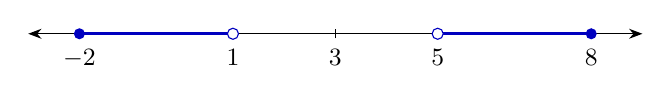
\begin{tikzpicture}[x=0.65cm,y=1cm,>=Stealth,font=\small]
            \draw[<->] (-3,0)--(9,0);
            \draw[blue!75!black,very thick] (-2,0)--(1,0);
            \draw[blue!75!black,very thick] (5,0)--(8,0);
            \foreach \x in {-2,1,3,5,8} {
                \draw (\x,-0.06)--(\x,0.06);
                \node[below] at (\x,-0.08) {$\x$};
              }
            \foreach \x in {-2,8} {\fill[blue!75!black] (\x,0) circle (2pt);}
            \foreach \x in {1,5} {\draw[blue!75!black,fill=white] (\x,0) circle (2pt);}
          \end{tikzpicture}
        \end{center}

        % Pembahasan soal 7
  \item Kedua garis berpotongan di $(4,-1)$, sehingga titik itu berada pada keduanya.
        Untuk garis yang tegak lurus, hasil kali gradiennya adalah $-1$:
        \[
          \frac23m_2=-1\quad\Longrightarrow\quad m_2=-\frac32.
        \]
        Gunakan bentuk titik--gradien:
        \[
          y+1=-\frac32(x-4)
          \quad\Longrightarrow\quad\boxed{l_2:y=-\frac32x+5}.
        \]
        Untuk menggambar $l_1$, gunakan gradien $\frac23$ dan titik yang sama:
        \[
          y+1=\frac23(x-4)
          \quad\Longrightarrow\quad l_1:y=\frac23x-\frac{11}{3}.
        \]
        Garis $l_1$ naik dari kiri ke kanan, sedangkan $l_2$ turun.
        Keduanya melewati $(4,-1)$ seperti pada sketsa.
        \begin{center}
          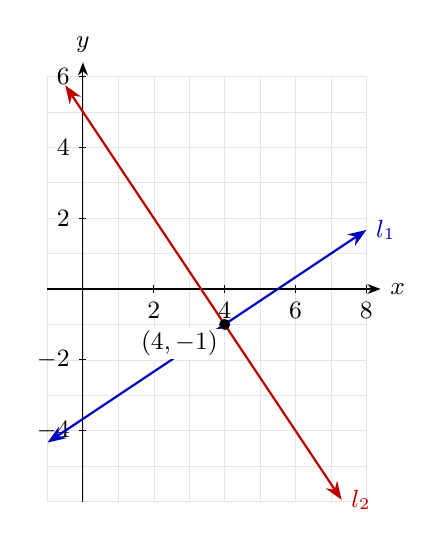
\begin{tikzpicture}[x=0.45cm,y=0.45cm,>=Stealth,font=\small]
            \draw[gray!20,very thin,step=1] (-1,-6) grid (8,6);
            \draw[->] (-1,0)--(8.4,0) node[right] {$x$};
            \draw[->] (0,-6)--(0,6.4) node[above] {$y$};
            \foreach \x in {2,4,6,8} {
                \draw (\x,-0.1)--(\x,0.1);
                \node[below] at (\x,-0.1) {$\x$};
              }
            \foreach \y in {-4,-2,2,4,6} {
                \draw (-0.1,\y)--(0.1,\y);
                \node[left] at (-0.1,\y) {$\y$};
              }
            \draw[blue!75!black,thick,<->,domain=-1:8,samples=2]
            plot (\x,{2*\x/3-11/3});
            \node[right,blue!75!black] at (8,1.67) {$l_1$};
            \draw[red!75!black,thick,<->,domain=-0.5:7.3,samples=2]
            plot (\x,{-3*\x/2+5});
            \node[right,red!75!black] at (7.3,-5.95) {$l_2$};
            \fill (4,-1) circle (2pt);
            \node[below left,fill=white,inner sep=1pt] at (3.9,-1.1) {$(4,-1)$};
          \end{tikzpicture}
        \end{center}

        \newpage

        % Pembahasan soal 8
  \item \begin{enumerate}
          \item Domain alami polinom $f$ adalah $\R$.
                Namun, pada seluruh $\R$, fungsi ini belum mempunyai invers sebagai fungsi.
                Sebagai contoh, $f(1)=f(3)=-3$, padahal masukannya berbeda.

                Lengkapi kuadrat untuk melihat bentuk parabolanya:
                \[
                  f(x)=x^2-4x=(x-2)^2-4.
                \]
                Puncaknya $(2,-4)$ dan sumbu simetrinya $x=2$.
                Agar setiap nilai keluaran memiliki tepat satu masukan, pilih satu sisi parabola.
                Salah satu pembatasan domain yang dapat dipakai adalah
                \[
                  \boxed{D_f=[2,\infty)}.
                \]
                Pada daerah ini, fungsi naik terus dan range-nya $[-4,\infty)$.
                Pilihan lain yang juga sah adalah $D_f=(-\infty,2]$.
                Pada sisi kiri ini, fungsi turun terus dan memiliki range yang sama.

          \item Gunakan pilihan $D_f=[2,\infty)$ terlebih dahulu.
                Misalkan $y=(x-2)^2-4$.
                Karena $x\ge2$, nilai $x-2$ tak negatif, sehingga pilih akar positif:
                \begin{align*}
                  y+4        & =(x-2)^2,      \\
                  \sqrt{y+4} & =x-2,          \\
                  x          & =2+\sqrt{y+4}.
                \end{align*}
                Tukar nama variabel untuk menulis rumus invers:
                \[
                  \boxed{f^{-1}(x)=2+\sqrt{x+4}}.
                \]
                Domain invers adalah range fungsi semula, yaitu $[-4,\infty)$.
                Range invers adalah domain fungsi semula, yaitu $[2,\infty)$.
                Jadi,
                \[
                  \boxed{D_{f^{-1}}=[-4,\infty),\qquad R_{f^{-1}}=[2,\infty)}.
                \]
                Jika pada (a) dipilih sisi kiri $D_f=(-\infty,2]$, maka $x-2\le0$.
                Cabang akarnya menjadi $x-2=-\sqrt{y+4}$.
                Untuk pilihan ini, hasilnya adalah
                \[
                  \boxed{f^{-1}(x)=2-\sqrt{x+4}},
                  \qquad D_{f^{-1}}=[-4,\infty),\quad R_{f^{-1}}=(-\infty,2].
                \]
                Tanda akar pada rumus invers harus mengikuti pembatasan domain yang dipilih.
        \end{enumerate}

        \newpage

        % Pembahasan soal 9
  \item \begin{enumerate}
          \item Nilai fungsi di $x=-3$ adalah $f(-3)=k$.
                Untuk memenuhi syarat soal, nilai ini harus sama dengan limit di sekitar $-3$.
                Untuk $x\ne-3$, faktorkan pembilang:
                \[
                  \frac{x^2-9}{x+3}
                  =\frac{(x-3)(x+3)}{x+3}=x-3.
                \]
                Pencoretan berlaku di sekitar $-3$, tetapi tidak pada $x=-3$ itu sendiri.
                Maka
                \[
                  \lim_{x\to-3}f(x)=\lim_{x\to-3}(x-3)=-3-3=-6.
                \]
                Agar nilai fungsi sama dengan limitnya, pilih $\boxed{k=-6}$.

          \item Untuk $x\ne-3$, telah diperoleh $f(x)=x-3$.
                Pada $x=-3$, nilai $k=-6$ juga sama dengan $x-3=-6$.
                Jadi, kedua cabang dapat digabung menjadi
                \[
                  \boxed{f(x)=x-3\quad\text{untuk setiap }x\in\R}.
                \]
                Fungsi ini merupakan polinom derajat satu.
        \end{enumerate}

        % Pembahasan soal 10
  \item Fungsi yang diberikan adalah pangkat lima dari fungsi lain.
        Misalkan fungsi dalamnya $u(x)=\sqrt{x}+2x^2+1$, sehingga $f(x)=u(x)^5$.
        Aturan rantai memberi
        \[
          f'(x)=5u(x)^4\,u'(x).
        \]
        Turunkan setiap suku pada fungsi dalam:
        \[
          u'(x)=\frac{d}{dx}\sqrt{x}+\frac{d}{dx}(2x^2)+\frac{d}{dx}(1)
          =\frac1{2\sqrt{x}}+4x.
        \]
        Ganti kembali $u(x)$ dengan rumusnya:
        \[
          \boxed{f'(x)=5\bigl(\sqrt{x}+2x^2+1\bigr)^4
            \left(\frac1{2\sqrt{x}}+4x\right),\qquad x>0}.
        \]
        Faktor pertama berasal dari turunan fungsi luar.
        Faktor kedua berasal dari turunan fungsi dalam.
        Syarat $x>0$ diperlukan pada rumus turunan karena penyebutnya memuat $\sqrt{x}$.

\end{enumerate}
\par\endgroup

\newpage

% Kelompok 3: lima soal
\begin{enumerate}

  % Soal 11
  \item \begin{enumerate}
          \item Definisikan $|3-x|$.
          \item Berdasarkan poin (a) tersebut tentukan semua nilai $x$ yang
                memenuhi persamaan
                \[
                  |3-x|\ge-2x+1.
                \]
        \end{enumerate}

        % Soal 12
  \item \begin{enumerate}
          \item Tentukan jarak titik $(1,3)$ dan $(7,11)$.
          \item Tentukan persamaan lingkaran yang diameternya adalah jarak titik
                $(1,3)$ ke $(7,11)$.
        \end{enumerate}

        % Soal 13
  \item Diberikan fungsi
        \[
          f(x)=
          \begin{cases}
            x-1,      & x<3,   \\
            2(x-4)^2, & x\ge3.
          \end{cases}
        \]
        \begin{enumerate}
          \item Dapatkan $f(3)$, $f(-2)$, dan $f(1-x^2)$.
          \item Dapatkan domain dan range dari $f(x)$.
          \item Sketsa grafik dari $f(x)$.
        \end{enumerate}

        % Soal 14
  \item Diberikan
        \[
          f(x)=\frac{x^3-1}{x-1}.
        \]
        \begin{enumerate}
          \item Dapatkan $\displaystyle\lim_{x\to1}f(x)$.
          \item Buatlah sketsa grafik $y=f(x)$.
        \end{enumerate}

        % Soal 15
  \item Diketahui kurva
        \[
          x^2y+4x-3y^2=2.
        \]
        \begin{enumerate}
          \item Dapatkan $\dfrac{dy}{dx}$ dengan menggunakan turunan fungsi implisit.
          \item Dari (a) dapatkan persamaan garis singgung pada kurva tersebut di titik $(1,1)$.
        \end{enumerate}

\end{enumerate}

\newpage
\begingroup
\fontsize{10.95}{13.5}\selectfont
\setlength{\parskip}{3pt}
\setlist[enumerate,1]{label=\arabic*.,leftmargin=25pt,itemsep=14pt,topsep=6pt,parsep=3pt}
\setlist[enumerate,2]{label=(\alph*),leftmargin=18pt,itemsep=8pt,topsep=5pt,parsep=3pt}
\textbf{\large Pembahasan}\par\medskip
\begin{enumerate}

  % Pembahasan soal 11
  \item \begin{enumerate}
          \item Jika $3-x\ge0$, atau $x\le3$, nilai di dalam mutlak tetap.
                Jika $3-x<0$, atau $x>3$, tandanya dibalik.
                Jadi,
                \[
                  \boxed{|3-x|=
                    \begin{cases}
                      3-x, & x\le3, \\
                      x-3, & x>3.
                    \end{cases}}
                \]

          \item \textbf{Kasus $x\le3$.} Gunakan $|3-x|=3-x$:
                \[
                  3-x\ge-2x+1\iff x+3\ge1\iff x\ge-2.
                \]
                Irisan dengan syarat $x\le3$ menghasilkan $[-2,3]$.

                \textbf{Kasus $x>3$.} Gunakan $|3-x|=x-3$:
                \[
                  x-3\ge-2x+1\iff3x\ge4\iff x\ge\frac43.
                \]
                Setiap $x>3$ sudah memenuhi $x\ge\frac43$.
                Jadi, hasil kasus kedua adalah $(3,\infty)$.
                Ambil gabungan kedua kasus:
                \[
                  \boxed{\mathrm{HP}=[-2,3]\cup(3,\infty)=[-2,\infty)}.
                \]
                Nilai $-2$ termasuk karena kedua ruas sama-sama bernilai $5$.
        \end{enumerate}

        % Pembahasan soal 12
  \item Misalkan kedua titik adalah $A(1,3)$ dan $B(7,11)$.
        \begin{enumerate}
          \item Selisih koordinatnya adalah $\Delta x=7-1=6$ dan $\Delta y=11-3=8$.
                Gunakan rumus jarak dari teorema Pythagoras:
                \[
                  AB=\sqrt{(\Delta x)^2+(\Delta y)^2}
                  =\sqrt{6^2+8^2}=\sqrt{100}=\boxed{10}.
                \]

          \item Kedua titik menjadi ujung diameter lingkaran.
                Pusat lingkaran adalah titik tengah diameter:
                \[
                  C=\left(\frac{1+7}{2},\frac{3+11}{2}\right)=\boxed{(4,7)}.
                \]
                Panjang diameter adalah $10$, sehingga jari-jarinya $r=10/2=5$.
                Gunakan bentuk baku $(x-h)^2+(y-k)^2=r^2$:
                \[
                  \boxed{(x-4)^2+(y-7)^2=25}.
                \]
                Kedua ujung diameter memang berada pada lingkaran.
                Misalnya, untuk $A$, diperoleh $(1-4)^2+(3-7)^2=9+16=25$.
        \end{enumerate}

        \newpage

        % Pembahasan soal 13
  \item \begin{enumerate}
          \item Pilih cabang fungsi berdasarkan nilai masukannya.
                Karena $3\ge3$, gunakan cabang kedua:
                \[
                  f(3)=2(3-4)^2=2(-1)^2=\boxed{2}.
                \]
                Karena $-2<3$, gunakan cabang pertama:
                \[
                  f(-2)=(-2)-1=\boxed{-3}.
                \]
                Pada $f(1-x^2)$, masukannya adalah seluruh bentuk $1-x^2$.
                Untuk setiap $x\in\R$, berlaku $x^2\ge0$, sehingga $1-x^2\le1<3$.
                Jadi, masukan ini selalu memakai cabang pertama:
                \[
                  f(1-x^2)=(1-x^2)-1=\boxed{-x^2}.
                \]

          \item Syarat $x<3$ dan $x\ge3$ mencakup seluruh bilangan real.
                Kedua rumus cabang juga berupa polinom, sehingga tidak ada pembatasan lain.
                Jadi, $\boxed{D_f=\R}$.

                Pada cabang pertama, $y=x-1$ dengan $x<3$ menghasilkan $y<2$.
                Range cabang ini adalah $(-\infty,2)$.
                Pada cabang kedua, $y=2(x-4)^2\ge0$.
                Nilai nol tercapai di $x=4$, dan nilainya meningkat tanpa batas saat $x$ membesar.
                Jadi, range cabang kedua adalah $[0,\infty)$.
                Gabungkan keduanya:
                \[
                  \boxed{R_f=(-\infty,2)\cup[0,\infty)=\R}.
                \]

          \item Gambar garis $y=x-1$ hanya untuk $x<3$.
                Lalu gambar parabola $y=2(x-4)^2$ hanya untuk $x\ge3$.
                Puncak parabolanya $(4,0)$.
                Kedua rumus bertemu di $(3,2)$.
                Titik itu diberi bulatan penuh karena termasuk melalui cabang kedua.
                \begin{center}
                  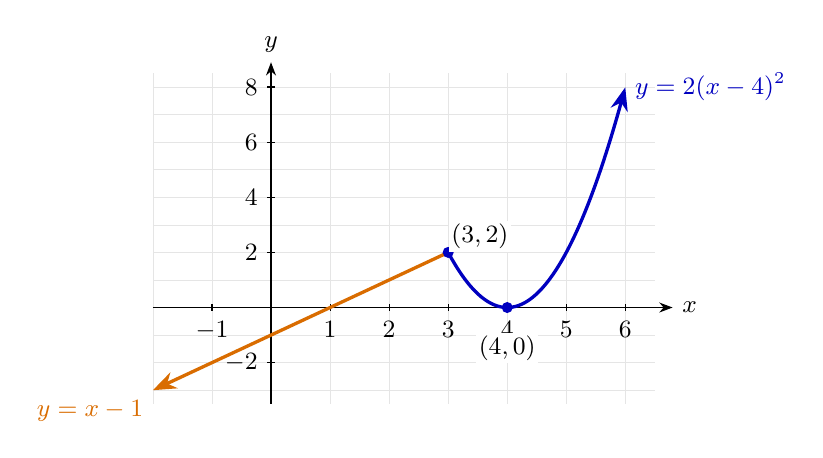
\begin{tikzpicture}[x=0.75cm,y=0.35cm,>=Stealth,font=\small]
                    \draw[gray!20,very thin,step=1] (-2,-3.5) grid (6.5,8.5);
                    \draw[->] (-2,0)--(6.8,0) node[right] {$x$};
                    \draw[->] (0,-3.5)--(0,8.9) node[above] {$y$};
                    \foreach \x in {-1,1,2,3,4,5,6} {
                        \draw (\x,-0.12)--(\x,0.12);
                        \node[below] at (\x,-0.15) {$\x$};
                      }
                    \foreach \y in {-2,2,4,6,8} {
                        \draw (-0.06,\y)--(0.06,\y);
                        \node[left] at (-0.06,\y) {$\y$};
                      }
                    \draw[orange!85!black,very thick,<-,domain=-2:3,samples=2]
                    plot (\x,{\x-1});
                    \node[below left,orange!85!black] at (-2,-3) {$y=x-1$};
                    \draw[blue!75!black,very thick,->,domain=3:6,samples=100,smooth]
                    plot (\x,{2*(\x-4)^2});
                    \node[right,blue!75!black] at (6,8) {$y=2(x-4)^2$};
                    \fill[blue!75!black] (3,2) circle (2pt);
                    \fill[blue!75!black] (4,0) circle (2pt);
                    \node[above right,fill=white,inner sep=1pt] at (3,2) {$(3,2)$};
                    \node[below,fill=white,inner sep=1pt] at (4,-0.9) {$(4,0)$};
                  \end{tikzpicture}
                \end{center}
        \end{enumerate}

        \newpage

        % Pembahasan soal 14
  \item \begin{enumerate}
          \item Substitusi langsung menghasilkan $0/0$.
                Gunakan pemfaktoran selisih kubus:
                \[
                  x^3-1=(x-1)(x^2+x+1).
                \]
                Untuk $x\ne1$, fungsi dapat disederhanakan menjadi
                \[
                  f(x)=\frac{(x-1)(x^2+x+1)}{x-1}=x^2+x+1.
                \]
                Saat menghitung limit, cukup tinjau nilai di sekitar $1$.
                Maka
                \[
                  \lim_{x\to1}f(x)=1^2+1+1=\boxed{3}.
                \]

          \item Grafik sama dengan parabola $y=x^2+x+1$, kecuali titik pada $x=1$.
                Titik $(1,3)$ harus dikosongkan karena fungsi semula tidak terdefinisi di sana.
                Bentuk puncaknya adalah
                \[
                  y=\left(x+\frac12\right)^2+\frac34.
                \]
                Jadi, puncaknya $(-\frac12,\frac34)$ dan parabola terbuka ke atas.
                Titik potong sumbu-$y$ adalah $(0,1)$.
                Tidak ada titik potong sumbu-$x$ karena nilai minimum parabolanya positif.
                \begin{center}
                  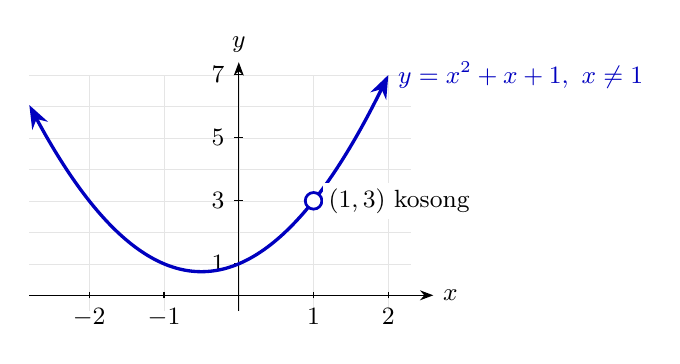
\begin{tikzpicture}[x=0.95cm,y=0.4cm,>=Stealth,font=\small]
                    \draw[gray!20,very thin,step=1] (-2.8,-0.5) grid (2.3,7);
                    \draw[->] (-2.8,0)--(2.6,0) node[right] {$x$};
                    \draw[->] (0,-0.5)--(0,7.4) node[above] {$y$};
                    \foreach \x in {-2,-1,1,2} {
                        \draw (\x,-0.1)--(\x,0.1);
                        \node[below] at (\x,-0.1) {$\x$};
                      }
                    \foreach \y in {1,3,5,7} {
                        \draw (-0.06,\y)--(0.06,\y);
                        \node[left] at (-0.06,\y) {$\y$};
                      }
                    \draw[blue!75!black,very thick,<->,domain=-2.8:2,samples=120,smooth]
                    plot (\x,{\x*\x+\x+1});
                    \node[right,blue!75!black] at (2,7) {$y=x^2+x+1,\ x\ne1$};
                    \draw[blue!75!black,fill=white,line width=1pt] (1,3) circle (3pt);
                    \node[right,fill=white,inner sep=2pt] at (1.12,3) {$(1,3)$ kosong};
                  \end{tikzpicture}
                \end{center}
        \end{enumerate}

        % Pembahasan soal 15
  \item \begin{enumerate}
          \item Anggap $y$ sebagai fungsi dari $x$.
                Suku $x^2y$ diturunkan dengan aturan hasil kali, sedangkan $y^2$ memakai aturan rantai:
                \[
                  \frac{d}{dx}(x^2y)=2xy+x^2y',\qquad
                  \frac{d}{dx}(y^2)=2yy'.
                \]
                Turunkan kedua ruas persamaan kurva:
                \begin{align*}
                  2xy+x^2y'+4-6yy' & =0,      \\
                  (x^2-6y)y'       & =-2xy-4.
                \end{align*}
                Dengan memisahkan $y'$, diperoleh
                \[
                  \boxed{\frac{dy}{dx}=\frac{2xy+4}{6y-x^2}}
                  \qquad(6y-x^2\ne0).
                \]

          \item Titik $(1,1)$ berada pada kurva karena $1+4-3=2$.
                Gradien garis singgung diperoleh dengan memasukkan titik ini ke turunan:
                \[
                  m=\left.\frac{dy}{dx}\right|_{(1,1)}
                  =\frac{2(1)(1)+4}{6(1)-1^2}=\frac65.
                \]
                Gunakan bentuk titik--gradien:
                \[
                  y-1=\frac65(x-1)
                  \quad\Longrightarrow\quad\boxed{6x-5y-1=0}.
                \]
        \end{enumerate}

\end{enumerate}
\par\endgroup

\newpage

% Kelompok 4: lima soal
\begin{enumerate}

  % Soal 16
  \item Dapatkan semua nilai $x$ yang memenuhi pertidaksamaan berikut:
        \[
          \frac{2x+1}{3x-6}<\frac12.
        \]

        % Soal 17
  \item Diberikan fungsi
        \[
          f(x)=\frac1{x-1}\quad\text{dan}\quad g(x)=2-\sqrt{x}.
        \]
        \begin{enumerate}
          \item Tentukan domain dari fungsi $f$ dan $g$.
          \item Dapatkan fungsi $(f\circ g)(x)$ beserta domainnya.
        \end{enumerate}

        % Soal 18
  \item Diberikan fungsi
        \[
          f(x)=
          \begin{cases}
            \dfrac{x^3-8}{2x-4}, & x\ne2, \\[5pt]
            k,                   & x=2.
          \end{cases}
        \]
        \begin{enumerate}
          \item Tentukan nilai $k$ sehingga $f(x)$ kontinu di $x=2$.
          \item Berdasarkan hasil dari (a), nyatakan $f(x)$ sebagai polinomial.
        \end{enumerate}

        % Soal 19
  \item Diberikan fungsi implisit
        \[
          3x^2+y^2-2xy+y-x=6.
        \]
        Tentukan $\dfrac{dy}{dx}$ di titik $(0,-3)$.

        % Soal 20
  \item Diketahui garis
        \[
          g_1:y=-x+6\quad\text{dan}\quad g_2:y=2x.
        \]
        \begin{enumerate}
          \item Tentukan titik potong kedua garis $g_1$ dan $g_2$.
          \item Tentukan titik potong $g_1$ dengan garis $x=1$.
                Tentukan pula titik potong $g_2$ dengan garis $x=1$.
          \item Gambarkan sketsa ketiga garis $g_1$, $g_2$, dan garis $x=1$.
                Hitung luas segitiga yang dibentuk ketiga garis tersebut.
        \end{enumerate}

\end{enumerate}

\newpage
\begingroup
\fontsize{10.95}{13.5}\selectfont
\setlength{\parskip}{3pt}
\setlist[enumerate,1]{label=\arabic*.,leftmargin=25pt,itemsep=14pt,topsep=6pt,parsep=3pt}
\setlist[enumerate,2]{label=(\alph*),leftmargin=18pt,itemsep=8pt,topsep=5pt,parsep=3pt}
\textbf{\large Pembahasan}\par\medskip
\begin{enumerate}

  % Pembahasan soal 16
  \item Syarat penyebut adalah $3x-6\ne0$, sehingga $x\ne2$.
        Pindahkan semua suku ke ruas kiri dan samakan penyebut:
        \begin{align*}
          \frac{2x+1}{3x-6}-\frac12      & <0, \\
          \frac{2(2x+1)-(3x-6)}{2(3x-6)} & <0, \\
          \frac{x+8}{6(x-2)}             & <0.
        \end{align*}
        Kita tidak langsung mengalikan dengan $3x-6$ karena tandanya bergantung pada $x$.
        Gunakan tabel tanda dengan titik batas $-8$ dan $2$:
        \[
          \begin{array}{c|ccc}
            x              & (-\infty,-8) & (-8,2) & (2,\infty) \\ \hline
            x+8            & -            & +      & +          \\
            x-2            & -            & -      & +          \\ \hline
            \text{pecahan} & +            & -      & +
          \end{array}
        \]
        Pecahan negatif hanya pada $-8<x<2$.
        Batas $-8$ tidak termasuk karena menghasilkan kesamaan, sedangkan $2$ membuat penyebut nol.
        Jadi, $\boxed{\mathrm{HP}=(-8,2)}$.

        % Pembahasan soal 17
  \item \begin{enumerate}
          \item Pada $f$, penyebut tidak boleh nol:
                \[
                  x-1\ne0\iff x\ne1,
                  \qquad\boxed{D_f=\R\setminus\{1\}}.
                \]
                Pada $g$, bilangan di dalam akar harus tak negatif.
                Karena itu, $x\ge0$, sehingga $\boxed{D_g=[0,\infty)}$.

          \item Masukkan $g(x)$ ke fungsi $f$:
                \[
                  (f\circ g)(x)=f(g(x))
                  =\frac1{g(x)-1}=\frac1{2-\sqrt{x}-1}
                  =\boxed{\frac1{1-\sqrt{x}}}.
                \]
                Domain komposisi harus memenuhi dua syarat.
                Fungsi dalam $g(x)$ harus terdefinisi, sehingga $x\ge0$.
                Hasil $g(x)$ juga harus berada dalam domain $f$, sehingga $g(x)\ne1$.
                Nilai yang membuat syarat kedua gagal adalah
                \[
                  2-\sqrt{x}=1\iff\sqrt{x}=1\iff x=1.
                \]
                Jadi, ambil semua $x\ge0$, lalu keluarkan $x=1$:
                \[
                  \boxed{D_{f\circ g}=[0,1)\cup(1,\infty)}.
                \]
                Nilai $0$ tetap termasuk karena penyebutnya $1-\sqrt0=1\ne0$.
        \end{enumerate}

        \newpage

        % Pembahasan soal 18
  \item \begin{enumerate}
          \item Kekontinuan di $x=2$ mensyaratkan nilai fungsi sama dengan limitnya.
                Karena $f(2)=k$, kita harus memilih $k=\lim_{x\to2}f(x)$.
                Faktorkan pembilang sebagai selisih kubus dan penyebut sebagai hasil kali:
                \[
                  x^3-8=(x-2)(x^2+2x+4),\qquad 2x-4=2(x-2).
                \]
                Untuk $x\ne2$,
                \[
                  f(x)=\frac{(x-2)(x^2+2x+4)}{2(x-2)}
                  =\frac{x^2+2x+4}{2}.
                \]
                Maka limitnya dapat dihitung dari polinom yang tersisa:
                \[
                  \lim_{x\to2}f(x)=\frac{2^2+2(2)+4}{2}
                  =\frac{12}{2}=6.
                \]
                Jadi, nilai yang membuat fungsi kontinu adalah $\boxed{k=6}$.

          \item Untuk $x\ne2$, fungsi sama dengan $\frac12x^2+x+2$.
                Pada $x=2$, polinom ini juga bernilai $\frac12(4)+2+2=6=k$.
                Karena kedua cabang sesuai pada seluruh domain, diperoleh
                \[
                  \boxed{f(x)=\frac12x^2+x+2\quad\text{untuk setiap }x\in\R}.
                \]
        \end{enumerate}

        % Pembahasan soal 19
  \item Titik $(0,-3)$ memang berada pada kurva karena $9-3=6$.
        Untuk menurunkan persamaan, anggap $y=y(x)$.
        Turunan $y^2$ adalah $2yy'$, sedangkan turunan $xy$ adalah $y+xy'$.
        Jadi,
        \begin{align*}
          6x+2yy'-2(y+xy')+y'-1 & =0,        \\
          6x+2yy'-2y-2xy'+y'-1  & =0,        \\
          (2y-2x+1)y'           & =-6x+2y+1.
        \end{align*}
        Maka
        \[
          \frac{dy}{dx}=\frac{-6x+2y+1}{2y-2x+1}.
        \]
        Masukkan koordinat $(0,-3)$:
        \[
          \left.\frac{dy}{dx}\right|_{(0,-3)}
          =\frac{-6(0)+2(-3)+1}{2(-3)-2(0)+1}
          =\frac{-5}{-5}=\boxed{1}.
        \]
        Penyebut di titik tersebut tidak nol, sehingga gradien ini terdefinisi.

        \newpage

        % Pembahasan soal 20
  \item \begin{enumerate}
          \item Pada titik potong kedua garis, nilai $x$ dan $y$ harus memenuhi kedua persamaan.
                Samakan kedua rumus $y$:
                \[
                  -x+6=2x\iff6=3x\iff x=2.
                \]
                Substitusikan ke $y=2x$, sehingga $y=4$.
                Jadi, titik potongnya adalah $\boxed{C(2,4)}$.

          \item Pada garis $x=1$, nilai koordinat $x$ sudah diketahui.
                Masukkan nilai ini ke masing-masing garis:
                \[
                  g_1:\quad y=-1+6=5,\qquad
                  g_2:\quad y=2(1)=2.
                \]
                Jadi, kedua titik potongnya adalah $\boxed{A(1,5)}$ dan $\boxed{B(1,2)}$.

          \item Segitiga dibentuk oleh titik $A$, $B$, dan $C$.
                Garis $g_1$ menurun, $g_2$ menaik, dan $x=1$ berupa garis vertikal.
                Daerah segitiga pada gambar diarsir agar batasnya terlihat jelas.
                \begin{center}
                  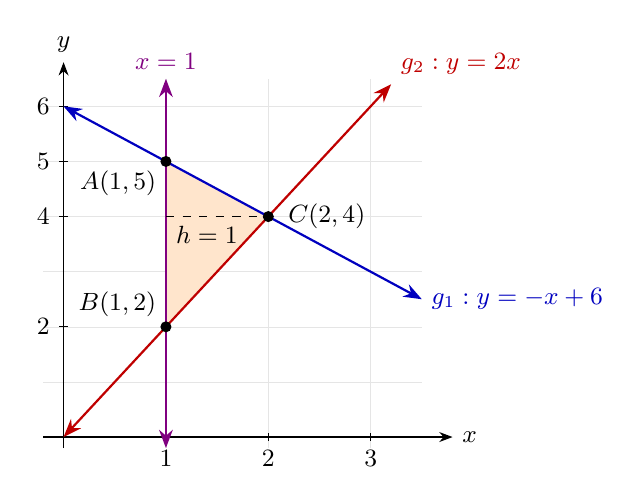
\begin{tikzpicture}[x=1.3cm,y=0.7cm,>=Stealth,font=\small]
                    \draw[gray!20,very thin,step=1] (-0.2,-0.2) grid (3.5,6.5);
                    \fill[orange!20] (1,5)--(1,2)--(2,4)--cycle;
                    \draw[->] (-0.2,0)--(3.8,0) node[right] {$x$};
                    \draw[->] (0,-0.2)--(0,6.8) node[above] {$y$};
                    \foreach \x in {1,2,3} {
                        \draw (\x,-0.07)--(\x,0.07);
                        \node[below] at (\x,-0.07) {$\x$};
                      }
                    \foreach \y in {2,4,5,6} {
                        \draw (-0.04,\y)--(0.04,\y);
                        \node[left] at (-0.04,\y) {$\y$};
                      }
                    \draw[blue!75!black,thick,<->,domain=0:3.5,samples=2]
                    plot (\x,{-\x+6});
                    \node[right,blue!75!black] at (3.5,2.5) {$g_1:y=-x+6$};
                    \draw[red!75!black,thick,<->,domain=0:3.2,samples=2]
                    plot (\x,{2*\x});
                    \node[above right,red!75!black] at (3.2,6.4) {$g_2:y=2x$};
                    \draw[violet,thick,<->] (1,-0.2)--(1,6.5);
                    \node[above,violet] at (1,6.5) {$x=1$};
                    \draw[black,dashed] (1,4)--(2,4);
                    \node[below] at (1.4,4) {$h=1$};
                    \foreach \p in {(1,5),(1,2),(2,4)} {\fill \p circle (2pt);}
                    \node[below left] at (1,5) {$A(1,5)$};
                    \node[above left] at (1,2) {$B(1,2)$};
                    \node[right] at (2.1,4) {$C(2,4)$};
                  \end{tikzpicture}
                \end{center}
                Pilih ruas vertikal $AB$ sebagai alas.
                Panjangnya adalah selisih koordinat $y$, yaitu $AB=5-2=3$.
                Tinggi segitiga adalah jarak tegak lurus dari $C(2,4)$ ke garis $x=1$.
                Karena alasnya vertikal, tinggi ini berupa jarak horizontal, yaitu $h=|2-1|=1$.
                Jadi,
                \[
                  \boxed{L=\frac12\cdot AB\cdot h
                    =\frac12\cdot3\cdot1=\frac32\text{ satuan luas}}.
                \]
        \end{enumerate}

\end{enumerate}
\par\endgroup

\end{document}
